\documentclass[12pt,twocolumn]{article}
\usepackage[T1]{fontenc}
\usepackage{graphicx}
\renewcommand*{\familydefault}{\sfdefault}
\title{\vspace{-2.5em}Investigation 1: Analytical Solutions}
\author{Christopher Pattison}
\date{}
\begin{document}
\maketitle
\newpage
\section*{Layout}
The program is laid out with a main body that handles all graphing with arrays being filled by subroutines containing the math. In this way, the mathematics are somewhat seperate from the graphing logic,
which allows significant modification to the underlying math without changing the body of the program. The subroutines take one or more pre-allocated arrays as well as function inputs.
\section*{Poisson's Equation}
Heat transfer in one dimension is a subroutine that contains hardcoded values for parameters such as boundary conditions and the source term.
\begin{figure}
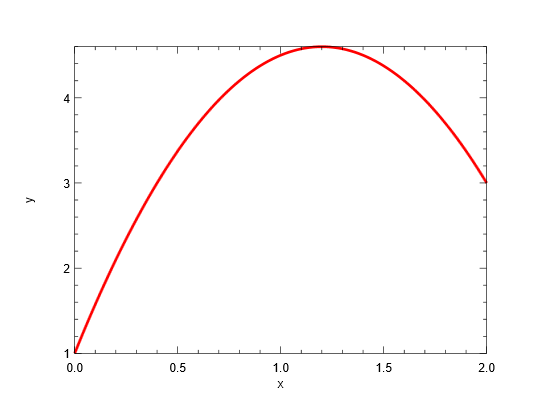
\includegraphics[width=\columnwidth]{1dheat.png}
\footnotesize{\caption{Poisson's Equation in 1D}}
\end{figure}
In two dimensions, a slight modification to the previous subroutine was made in the addition of a two dimensional result array and a second one dimensional function input. The result array is filled element-wise by a math function $f(x,y)$ that is the solution to the 
2D heat equation. Additionally, the first 41 terms of the infinite sum in the solution are taken in an inline loop. Repetitive terms 
in the sum were moved to another function for brevity.
\begin{figure}
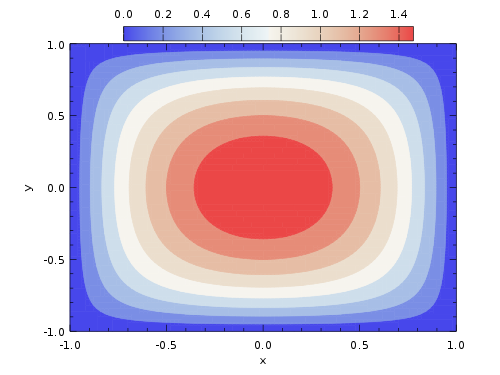
\includegraphics[width=\columnwidth]{2dheat.png}
\footnotesize{\caption{Poisson's Equation in 2D}}
\end{figure}
\section*{Vortex}
A vortex in 2D is implemented by a subroutine that takes arrays of x and y coordinates as well as a three dimensional array. The 
first dimension is the components of the vector which is filled component-wise. The Fortran ternary intrinsic \emph{merge} proved 
useful to implement the piecewise velocity distribution. Array slicing was used to seperate the vector into its components as required 
for graphing.
\begin{figure}
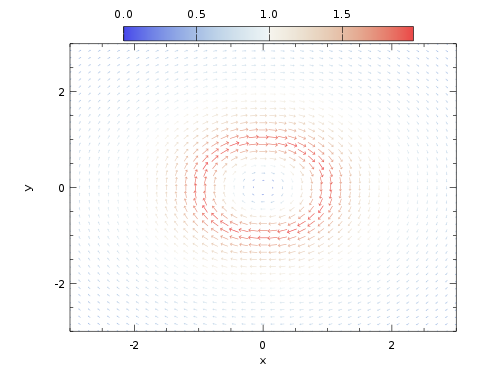
\includegraphics[width=\columnwidth]{vortex.png}
\footnotesize{\caption{Vortex}}
\end{figure}
\section*{Vortex Smoothing}
The velocity distribution being only $C^0$ continuous and unrealistic makes it desirable to fit a polynomial in its place. A system of equations is generated based on sampling points that can either be
supplied or generated with a linear distribution. If a linear distribution is desired, an array of size other than \emph{order$+1$} is provided. 
The system is solved using Gaussian Elimination, zeroing out first the lower and then the upper half using row operations.
The row operations are computed by using array slicing to handle an entire row at once, significantly reducing the amount of code required. The fitted values are then calculated by summing the second rank resulting from an inline loop and subsequent reshape.
\begin{figure}
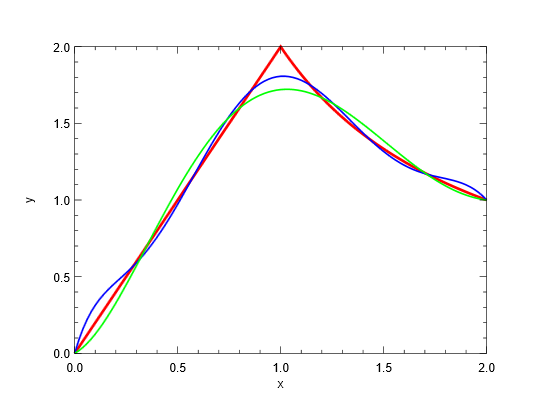
\includegraphics[width=\columnwidth]{vortexvel.png}
\footnotesize{\caption{Vortex Velocity Distribution}}
\end{figure}
A 3th order polynomial proved to provide the best fit when the sampling points were hand picked whereas a 5th order polynomial was more appropriate with evenly distributed sampling points.
\end{document}
